\documentclass{beamer}
\usepackage{tcolorbox}
\usepackage{amsmath}
\usepackage{tikz}
\usepackage{pgfplots}
\usepackage{adjustbox}

%\beamerdefaultoverlayspecification{<+->}
\newcommand{\data}{\mathcal{D}}

\DeclareMathOperator*{\argmin}{arg\,min}

\newcommand\Item[1][]{%
	\ifx\relax#1\relax  \item \else \item[#1] \fi
	\abovedisplayskip=0pt\abovedisplayshortskip=0pt~\vspace*{-\baselineskip}}


\usetheme{metropolis}           % Use metropolis theme


\title{Gradient Descent}
\date{\today}
\author{Nipun Batra}
\institute{IIT Gandhinagar}
\begin{document}
	\maketitle
	
	
	\begin{frame}{Data}
		
		\begin{center}
			\begin{tabular}{|c|c|}
				\hline
				\hline
				x&y  \\
				\hline
				1&1\\
				2&2\\
				3&3\\
				\hline
			\end{tabular}\\
			
		\end{center}
		
		% $\hat{y} = \theta_{0} + \theta_{1}x$\\
		% \epsilon_{i} = y_{i} = \hat{y_{i}}\\
		% \begin{itemize}
		%     \item $\epsilon_{1} = 1 - \theta_{0} - \theta_{1}$
		%     \item $\epsilon_{2} = 2 - \theta_{0} - 2\theta_{1}$
		%     \item $\epsilon_{3} = 3 - \theta_{0} - 3\theta_{1}$
		% \end{itemize}
	\end{frame}
	
	% \section{Linear Regression}
	
	\begin{frame}{Cost Function}
		The following denote the cost function for the above examples
		
		\begin{itemize}
			\item $\epsilon_{1} =1 -  \theta_{0} - \theta_{1}$
			\item $\epsilon_{2} =2 -  \theta_{0} - 2\theta_{1}$
			\item $\epsilon_{3} =3 -  \theta_{0} - 3\theta_{1}$
		\end{itemize}
		
		$\sum \epsilon_{i}^{2}$ = $14+3\theta_{0}^{2}+14\theta_{1}^{2}-12\theta_{0}-28\theta_{1}+12\theta_{0}\theta_{1}$
	\end{frame}
	

\begin{frame}{Contour Plot}
	
	$\sum \epsilon_{i}^{2}$ = $14+3\theta_{0}^{2}+14\theta_{1}^{2}-12\theta_{0}-28\theta_{1}+12\theta_{0}\theta_{1}$\\
	
	\begin{columns}
		\pause \begin{column}{0.6\textwidth}
			\begin{adjustbox}{max totalsize={\textwidth},center}
				
				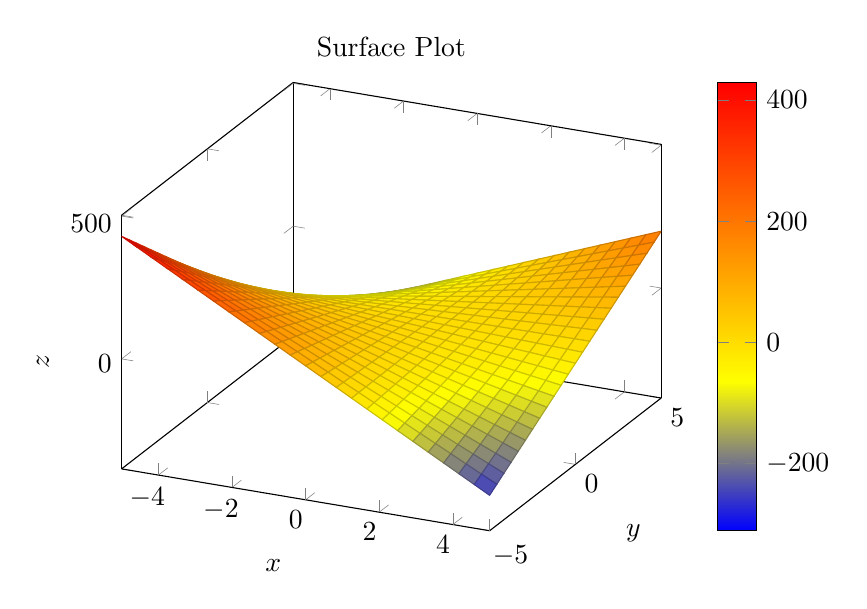
\begin{tikzpicture}
				\begin{axis}[colorbar,xlabel=$x$, ylabel=$y$, zlabel=$z$,title={Surface Plot}]
				\addplot3[
				surf,
				]
				{14 + 3*x +14*y -12*x - 28*y + 12*x*y};
				\end{axis}
				\end{tikzpicture}
			\end{adjustbox}
			
		\end{column}
		\pause \begin{column}{0.5\textwidth}
			\begin{adjustbox}{max totalsize={\textwidth},center}
				\begin{tikzpicture}
				\begin{axis}
				[
				title={Contour plot, view from top},
				view={0}{90},
				xlabel=$x$,
				ylabel=$y$,
				axis x line*=bottom,
				axis y line*=left,
				xtick align=outside,
				ytick align=outside,
				unit vector ratio*=1 1 1,
				]
				\addplot3[
				contour gnuplot={number=14,}
				]
				{14 + 3*x +14*y -12*x - 28*y + 12*x*y};
				\end{axis}
				\end{tikzpicture}
			\end{adjustbox}
		\end{column}
	\end{columns}
	

	
	
\end{frame}



	\begin{frame}{Gradient Descent for Parabola }
		Start with a random starting point for x.\\ Say x = 4.1\\
		$\cfrac{\partial}{\partial x}(x^2) = 2x$
		
		\begin{itemize}
			\item<+-> $x = 4.10 - \alpha * 2 * 4.10 $; $x = 3.68$
			\item<+-> $x = 3.68 - \alpha * 2 *3.68 $; $x = 3.32$
			\item<+-> $x = 3.32 - \alpha * 2 *3.32 $; $x = 2.98$
			\item<+-> \dots
		\end{itemize}
		
		
	\end{frame}
	
	\begin{frame}{Gradient Descent}
		\begin{center}
			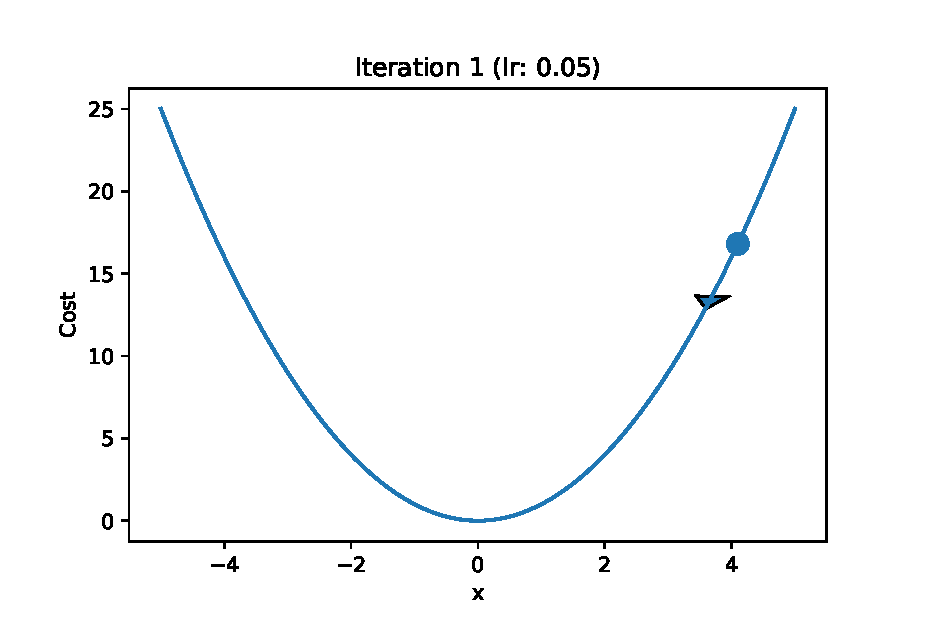
\includegraphics[totalheight=6cm]{gradient-descent/iteration-1.eps}
		\end{center}
	\end{frame}
	
	\begin{frame}{Gradient Descent}
		\begin{center}
			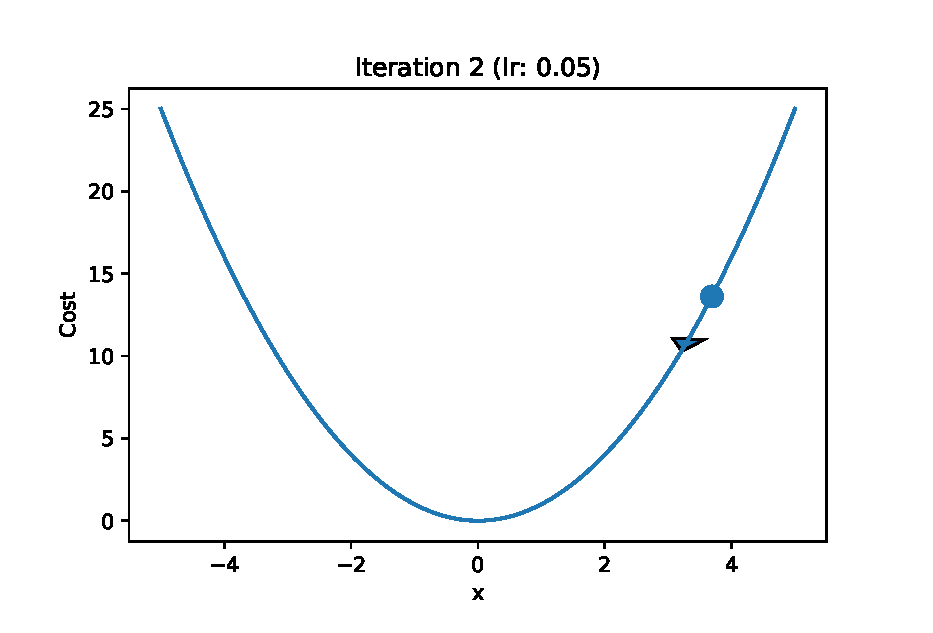
\includegraphics[totalheight=6cm]{gradient-descent/iteration-2.eps}
		\end{center}
	\end{frame}
	
	\begin{frame}{Gradient Descent}
		\begin{center}
			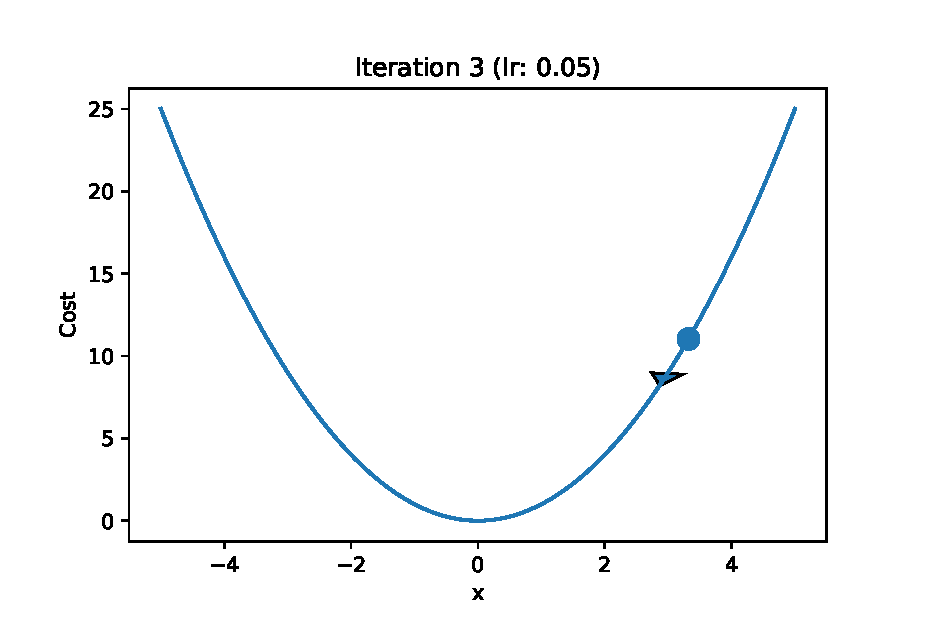
\includegraphics[totalheight=6cm]{gradient-descent/iteration-3.eps}
		\end{center}
	\end{frame}
	
	\begin{frame}{Gradient Descent}
		\begin{center}
			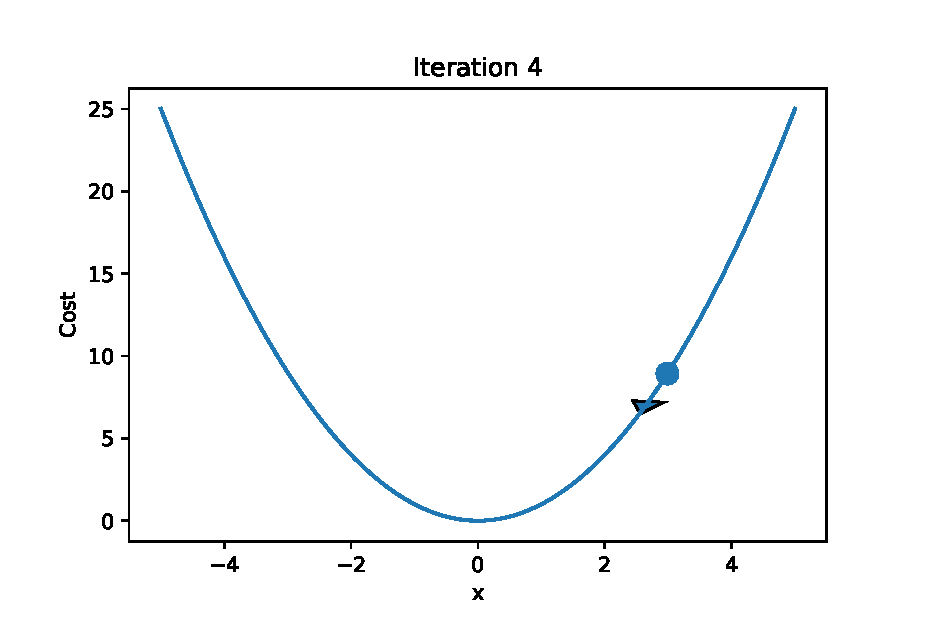
\includegraphics[totalheight=6cm]{gradient-descent/iteration-4.eps}
		\end{center}
	\end{frame}
	
	\begin{frame}{Gradient Descent}
		\begin{center}
			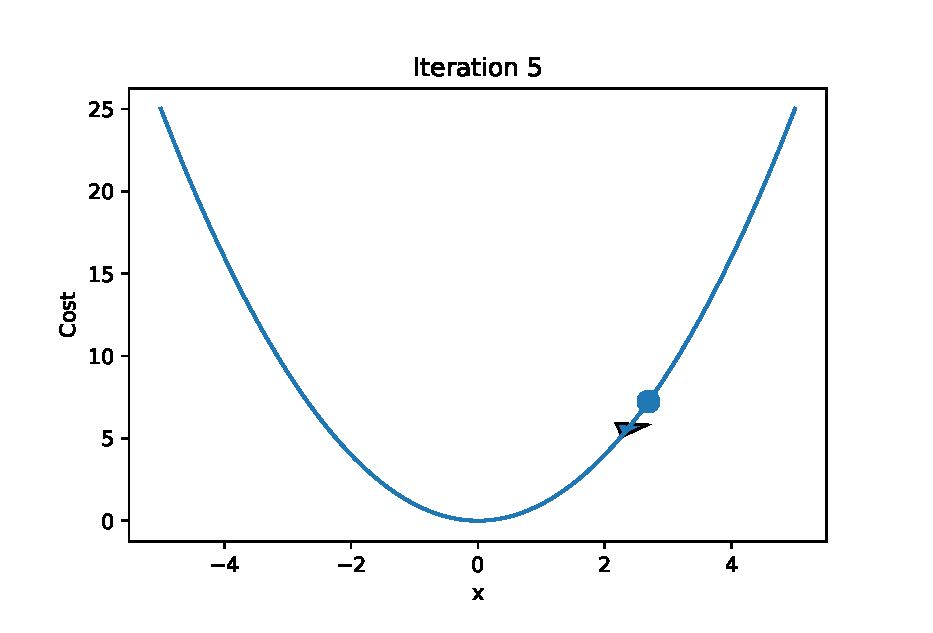
\includegraphics[totalheight=6cm]{gradient-descent/iteration-5.eps}
		\end{center}
	\end{frame}
	
	\begin{frame}{Gradient Descent}
		\begin{center}
			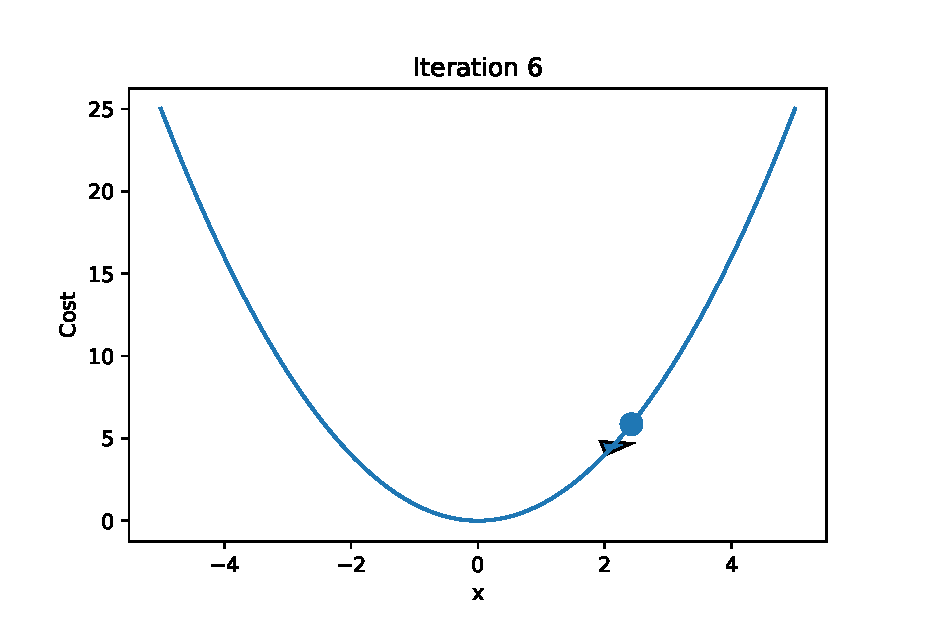
\includegraphics[totalheight=6cm]{gradient-descent/iteration-6.eps}
		\end{center}
	\end{frame}
	
	\begin{frame}{Gradient Descent}
		\begin{center}
			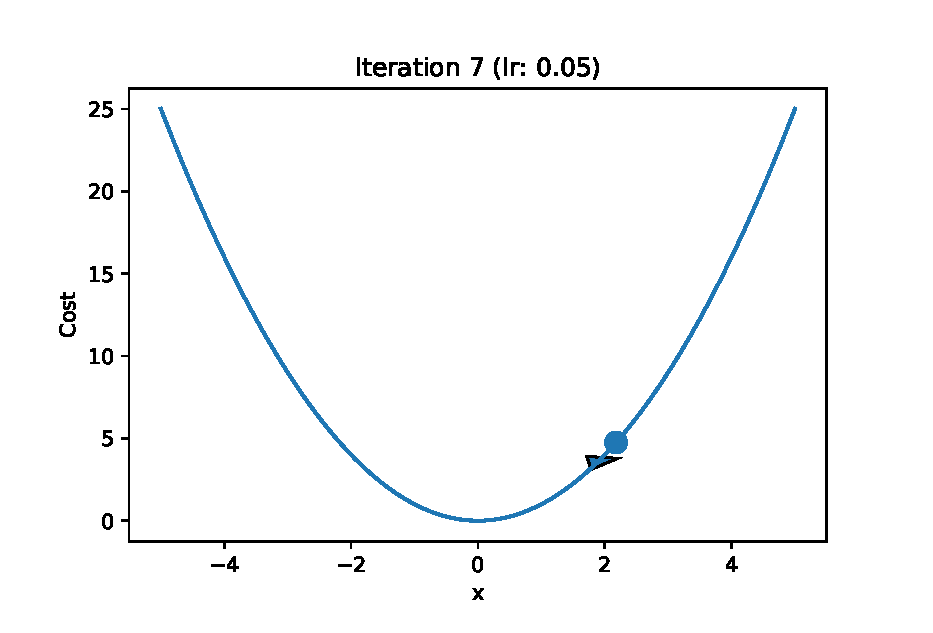
\includegraphics[totalheight=6cm]{gradient-descent/iteration-7.eps}
		\end{center}
	\end{frame}
	
	\begin{frame}{Gradient Descent}
		\begin{center}
			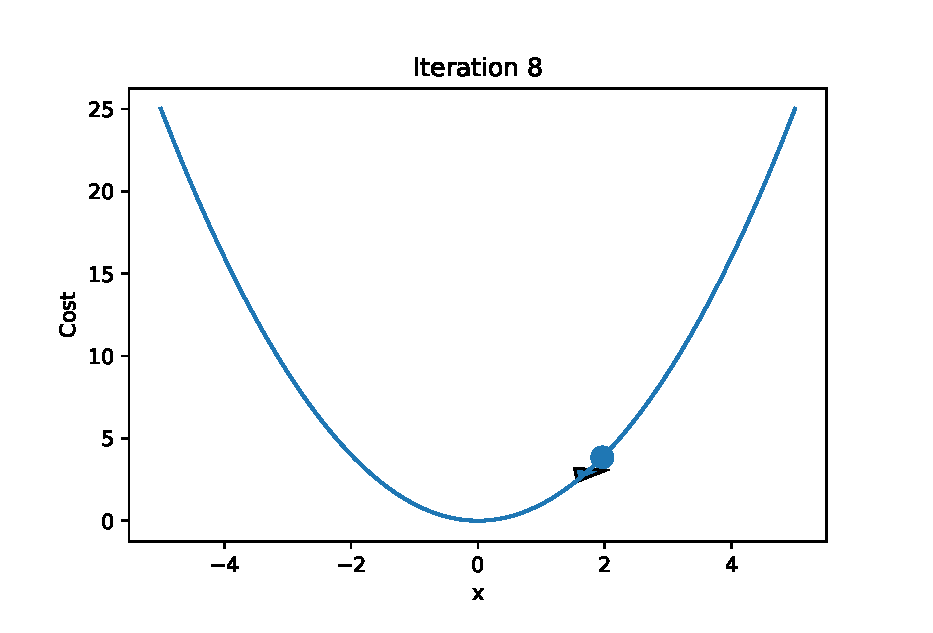
\includegraphics[totalheight=6cm]{gradient-descent/iteration-8.eps}
		\end{center}
	\end{frame}
	
	\begin{frame}{Gradient Descent}
		\begin{center}
			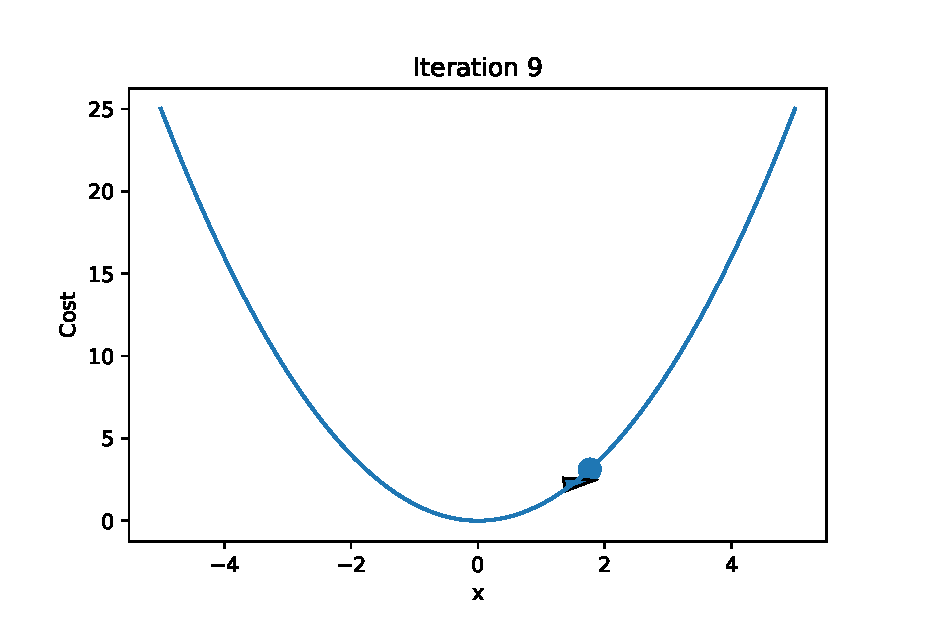
\includegraphics[totalheight=6cm]{gradient-descent/iteration-9.eps}
		\end{center}
	\end{frame}
	
	\begin{frame}{Gradient Descent}
		\begin{center}
			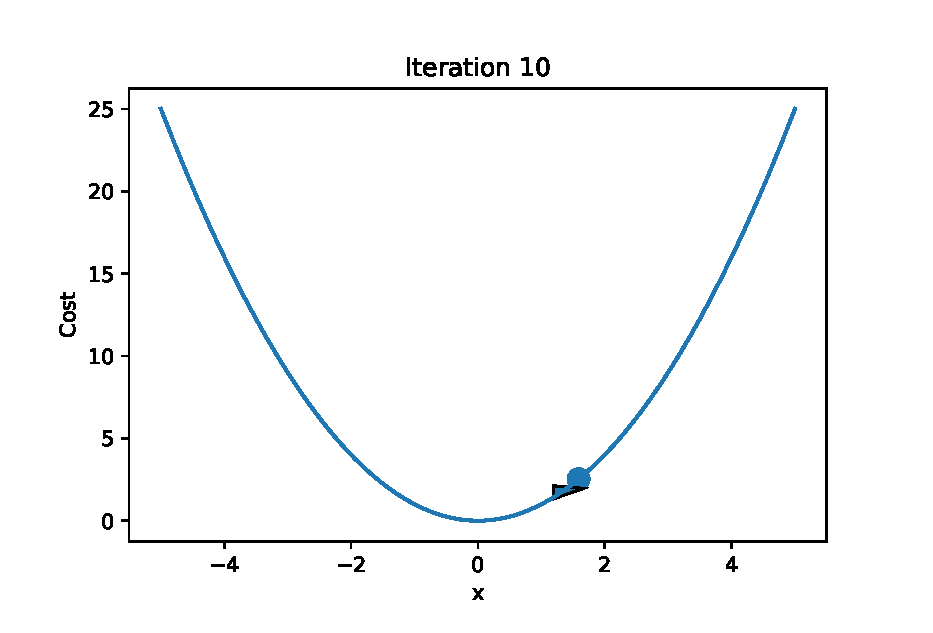
\includegraphics[totalheight=6cm]{gradient-descent/iteration-10.eps}
		\end{center}
	\end{frame}
	
	\begin{frame}{Gradient Descent}
		\begin{center}
			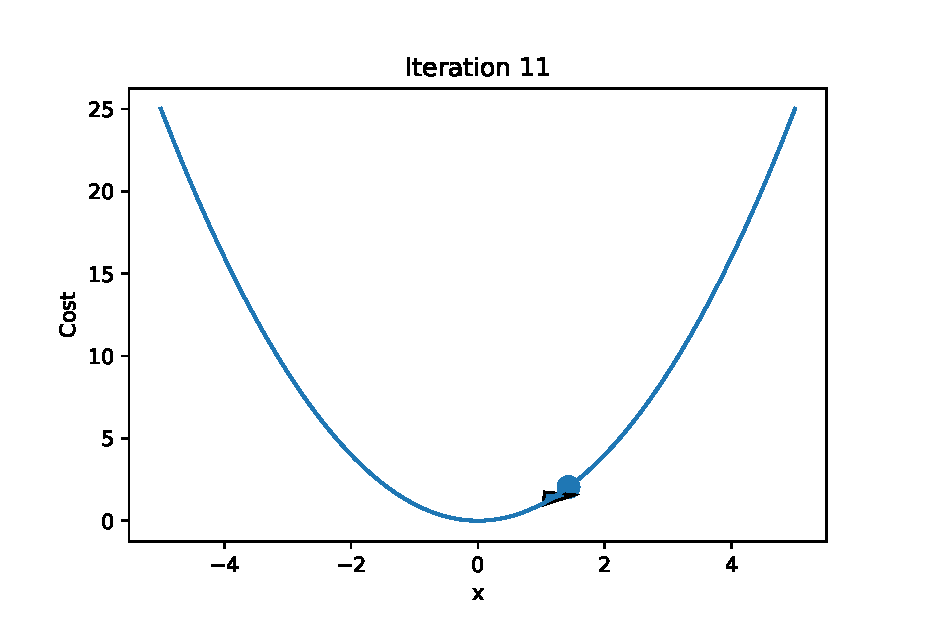
\includegraphics[totalheight=6cm]{gradient-descent/iteration-11.eps}
		\end{center}
	\end{frame}
	
	\begin{frame}{Gradient Descent}
		\begin{center}
			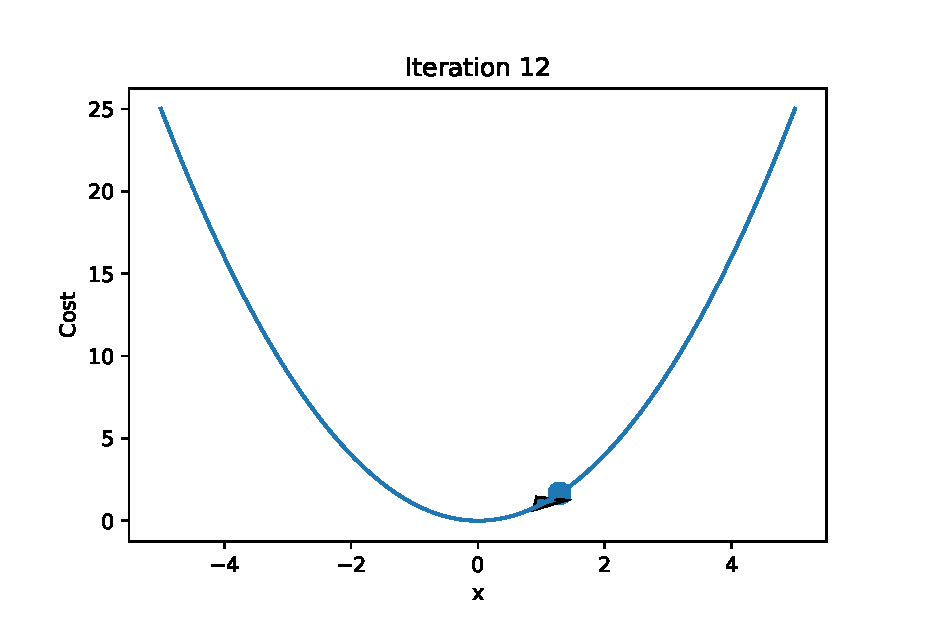
\includegraphics[totalheight=6cm]{gradient-descent/iteration-12.eps}
		\end{center}
	\end{frame}
	
	\begin{frame}{Gradient Descent}
		\begin{center}
			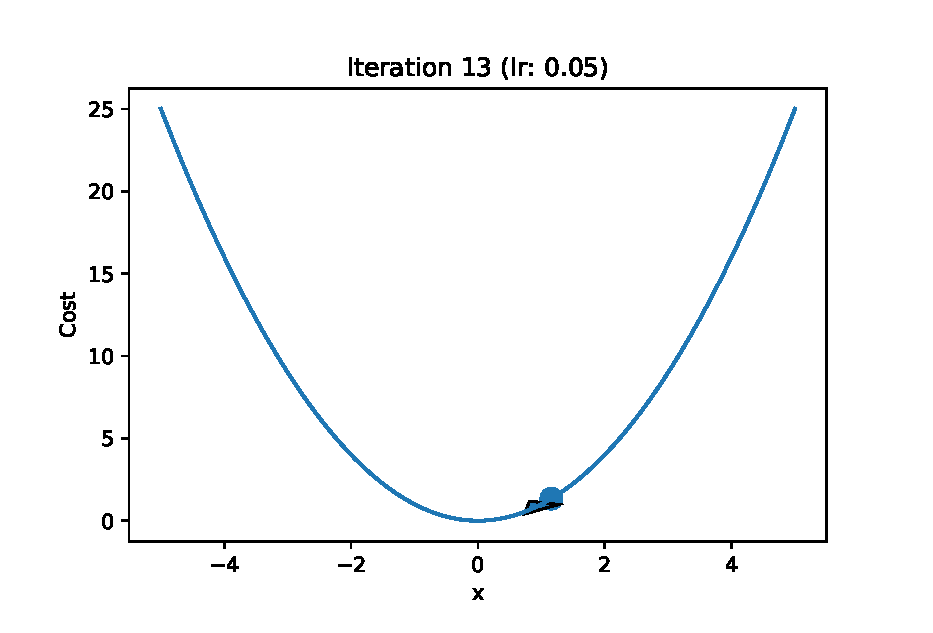
\includegraphics[totalheight=6cm]{gradient-descent/iteration-13.eps}
		\end{center}
	\end{frame}
	
	\begin{frame}{Gradient Descent}
		\begin{center}
			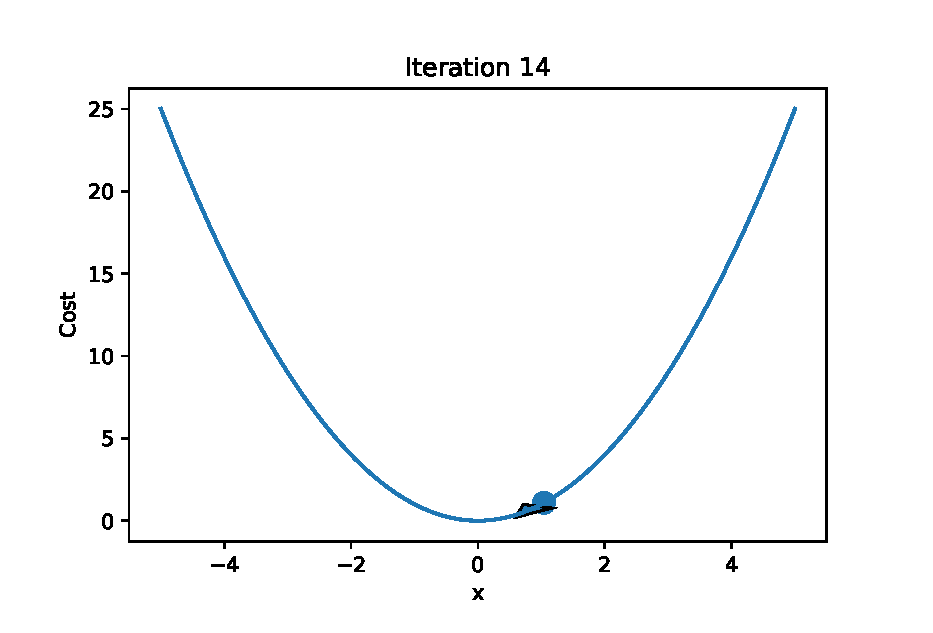
\includegraphics[totalheight=6cm]{gradient-descent/iteration-14.eps}
		\end{center}
	\end{frame}
	
	\begin{frame}{Gradient Descent}
		\begin{center}
			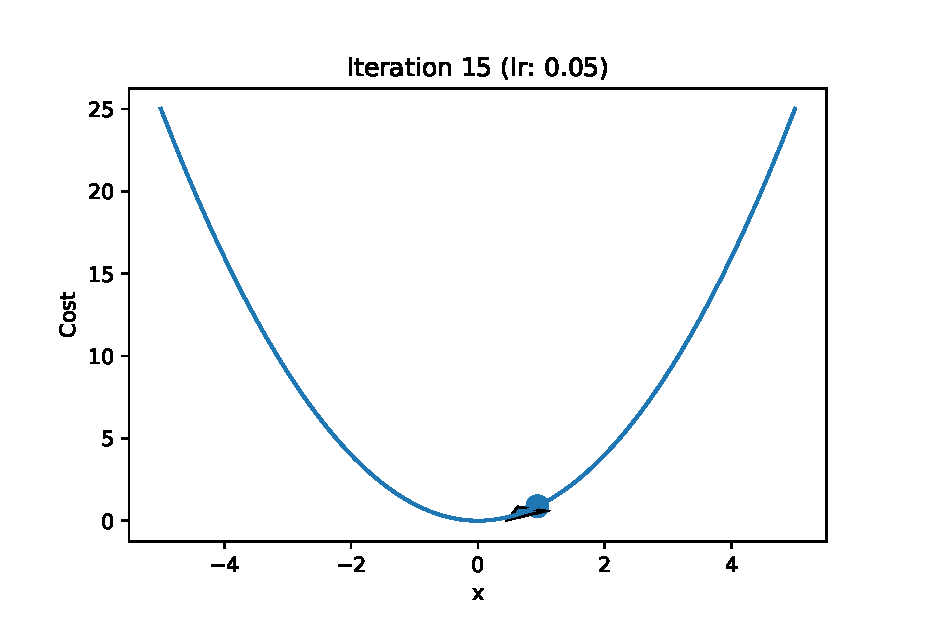
\includegraphics[totalheight=6cm]{gradient-descent/iteration-15.eps}
		\end{center}
	\end{frame}
	
	\begin{frame}{Gradient Descent}
		\begin{center}
			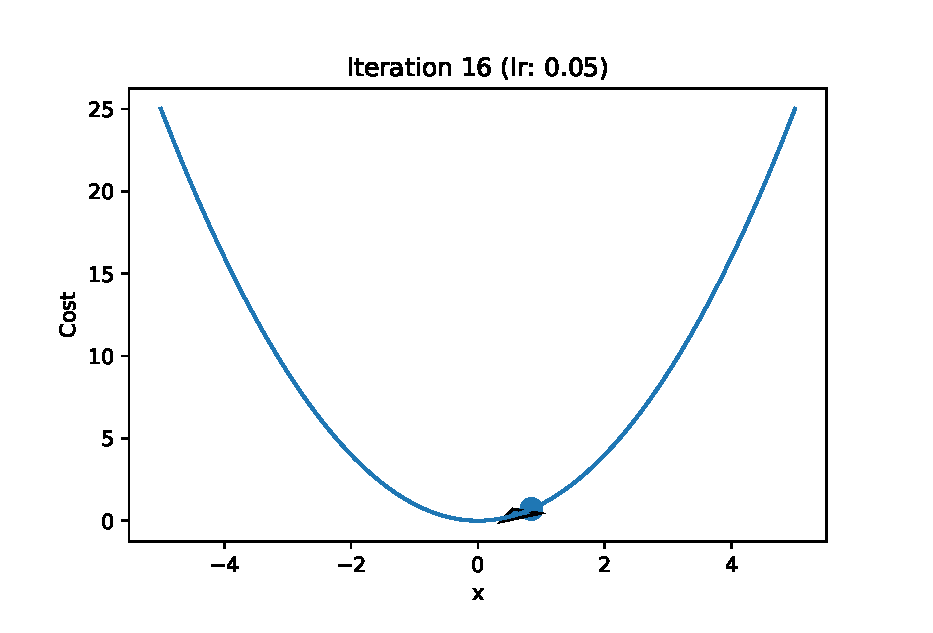
\includegraphics[totalheight=6cm]{gradient-descent/iteration-16.eps}
		\end{center}
	\end{frame}
	
	\begin{frame}{Gradient Descent}
		\begin{center}
			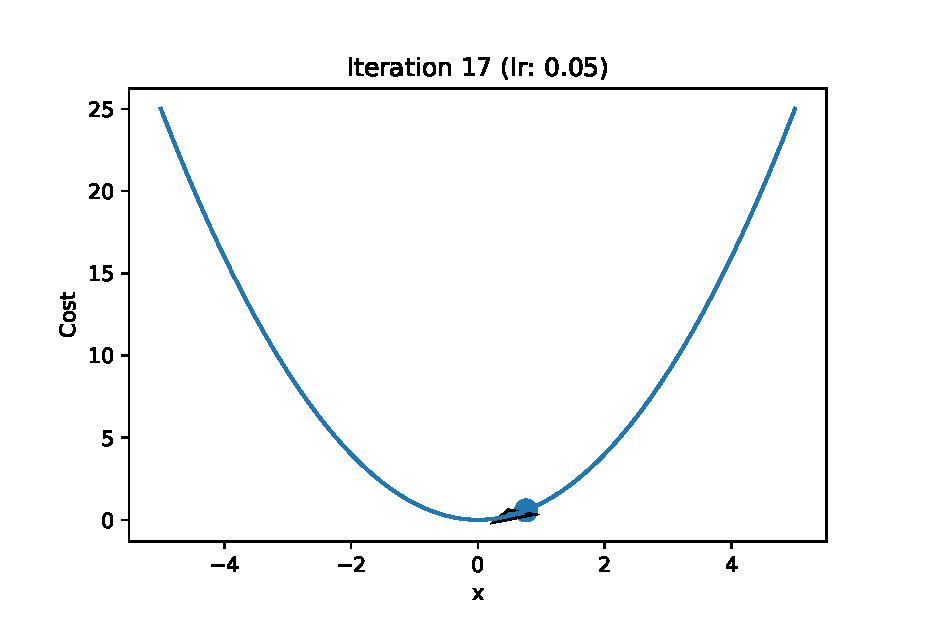
\includegraphics[totalheight=6cm]{gradient-descent/iteration-17.eps}
		\end{center}
	\end{frame}
	
	\begin{frame}{Gradient Descent}
		\begin{center}
			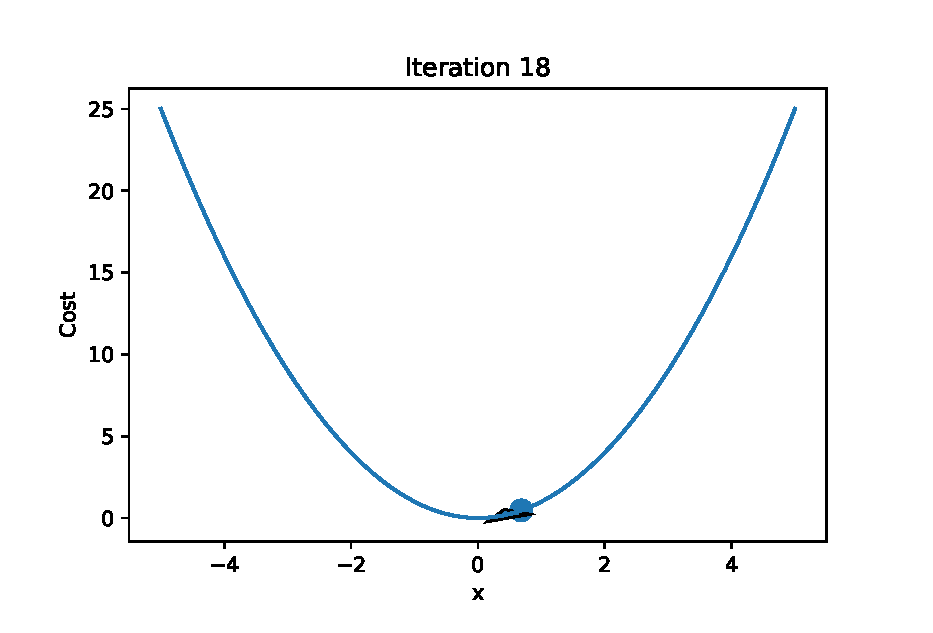
\includegraphics[totalheight=6cm]{gradient-descent/iteration-18.eps}
		\end{center}
	\end{frame}
	
	\begin{frame}{Gradient Descent}
		\begin{center}
			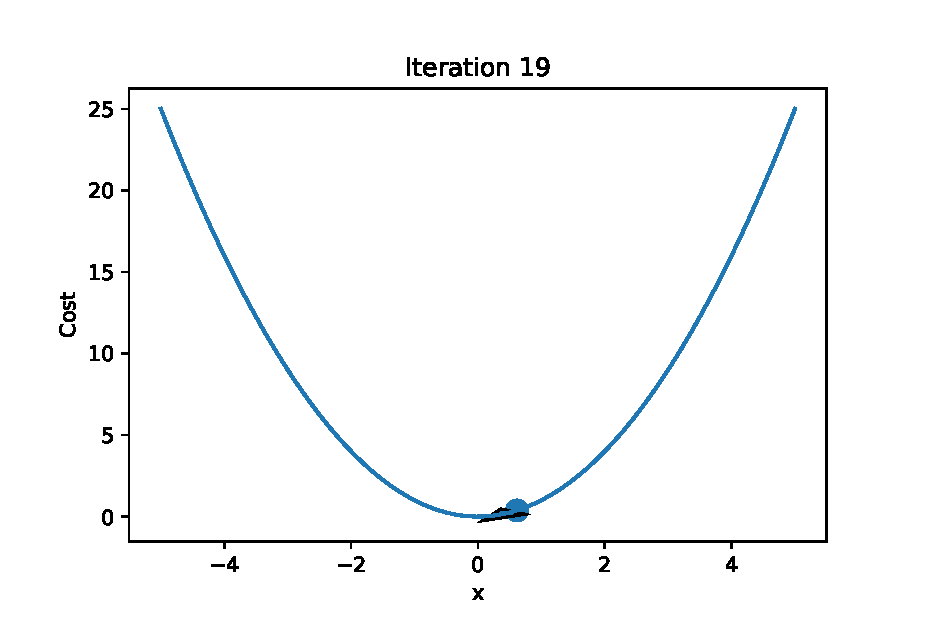
\includegraphics[totalheight=6cm]{gradient-descent/iteration-19.eps}
		\end{center}
	\end{frame}
	
	\begin{frame}{Gradient Descent}
		\begin{center}
			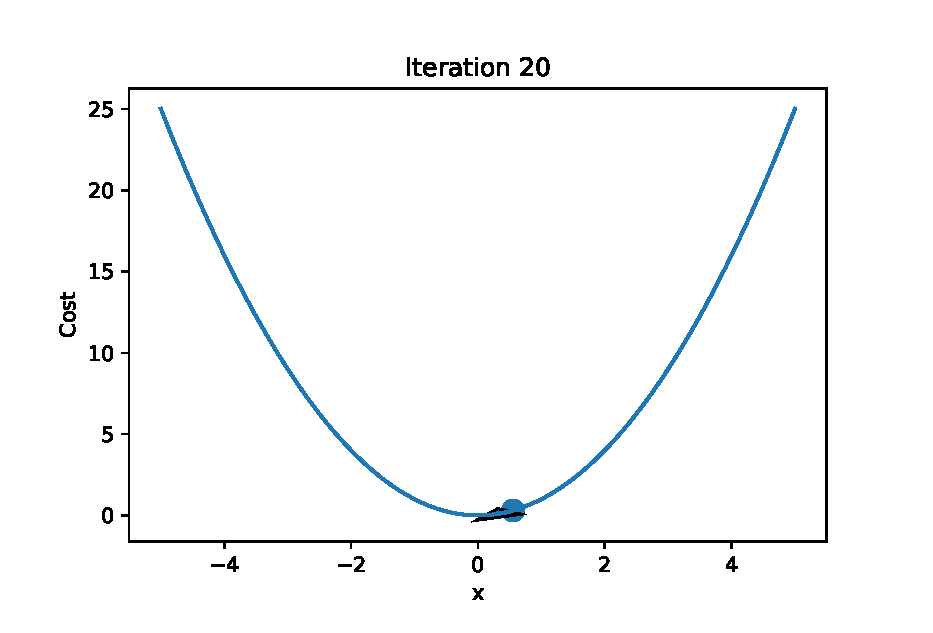
\includegraphics[totalheight=6cm]{gradient-descent/iteration-20.eps}
		\end{center}
	\end{frame}
	
	
	
	\begin{frame}{Gradient Descent}
		General Optimization Technique\\
		Question: Find minimum y
	\end{frame}
	
	\begin{frame}{Gradient Descent}
		General Optimization Technique\\
		Question: Find minimum y
		\begin{itemize}
			\item Start with some $x_{0}$
			\item Go to $x_{1}$ from $x_{0} $ such that $y_{1}< y_{0}$
		\end{itemize}
		
		\begin{equation*}
		x_{i} = x_{i-1} - \alpha\frac{\partial y }{\partial x} x_{i-1}
		\end{equation*}
		
	\end{frame}
	
	\begin{frame}{Local Minima}
		\begin{center}
			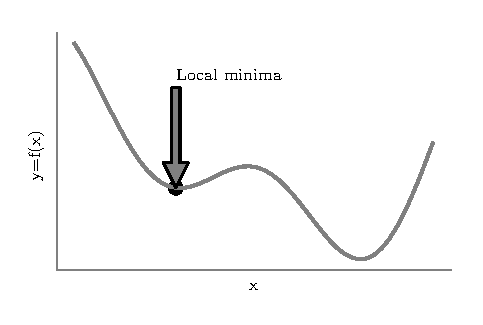
\includegraphics[totalheight=6cm]{gradient-descent/local-minima.eps}
		\end{center}
	\end{frame}
	
	
	
	
	\begin{frame}{What if $\alpha$ is large?}
		The model starts overshooting!
	\end{frame}
	
	\begin{frame}{Overshooting}
		\begin{center}
			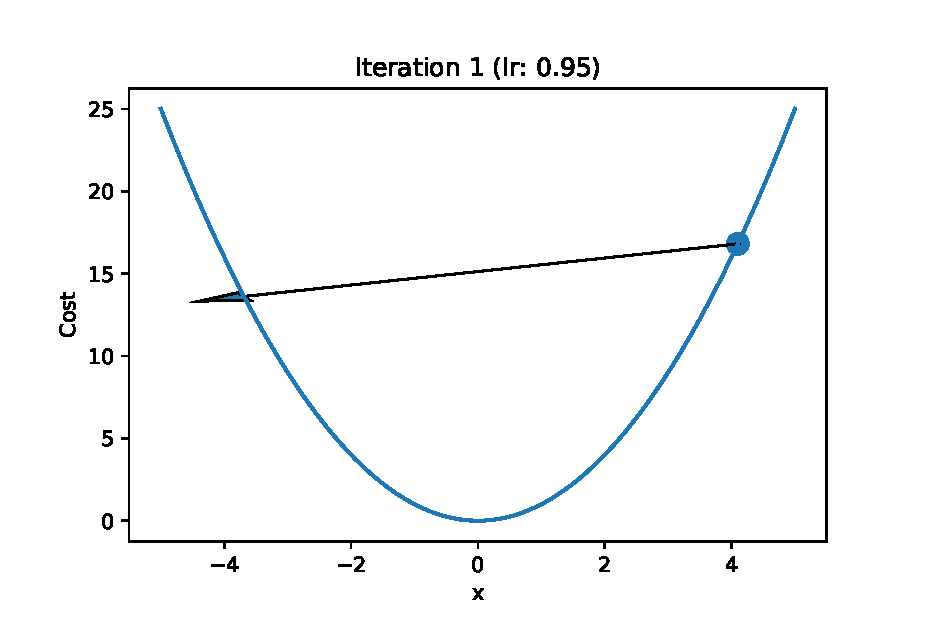
\includegraphics[totalheight=6cm]{gradient-descent/overshooting-1.eps}
		\end{center}
	\end{frame}
	
	\begin{frame}{Overshooting}
		\begin{center}
			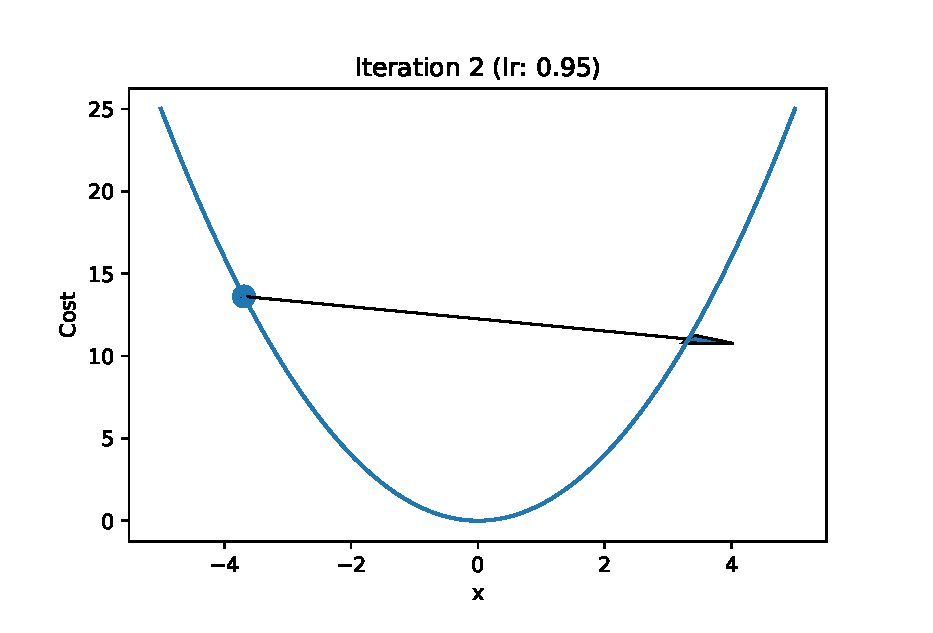
\includegraphics[totalheight=6cm]{gradient-descent/overshooting-2.eps}
		\end{center}
	\end{frame}
	
	\begin{frame}{Overshooting}
		\begin{center}
			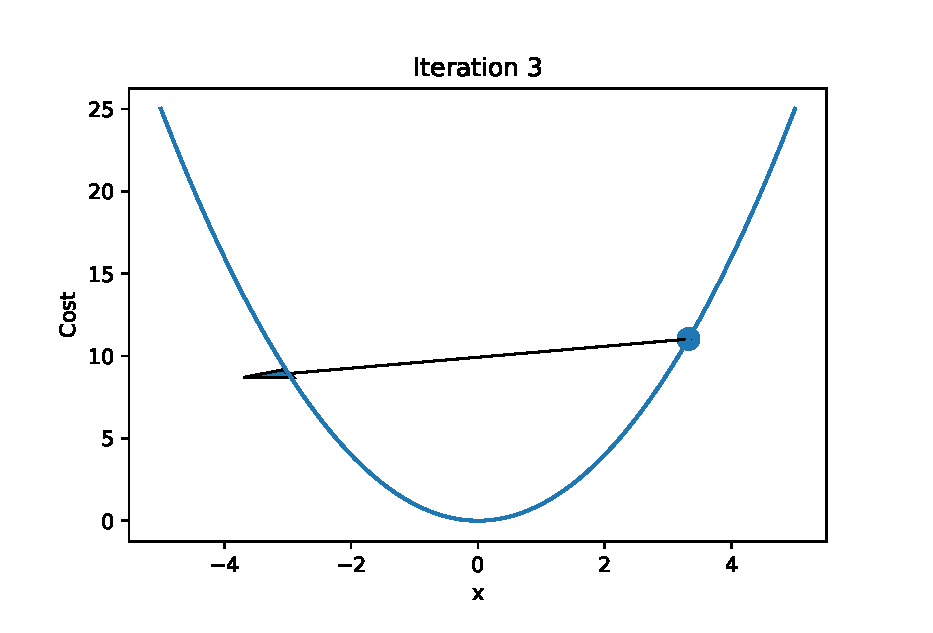
\includegraphics[totalheight=6cm]{gradient-descent/overshooting-3.eps}
		\end{center}
	\end{frame}
	
	\begin{frame}{Overshooting}
		\begin{center}
			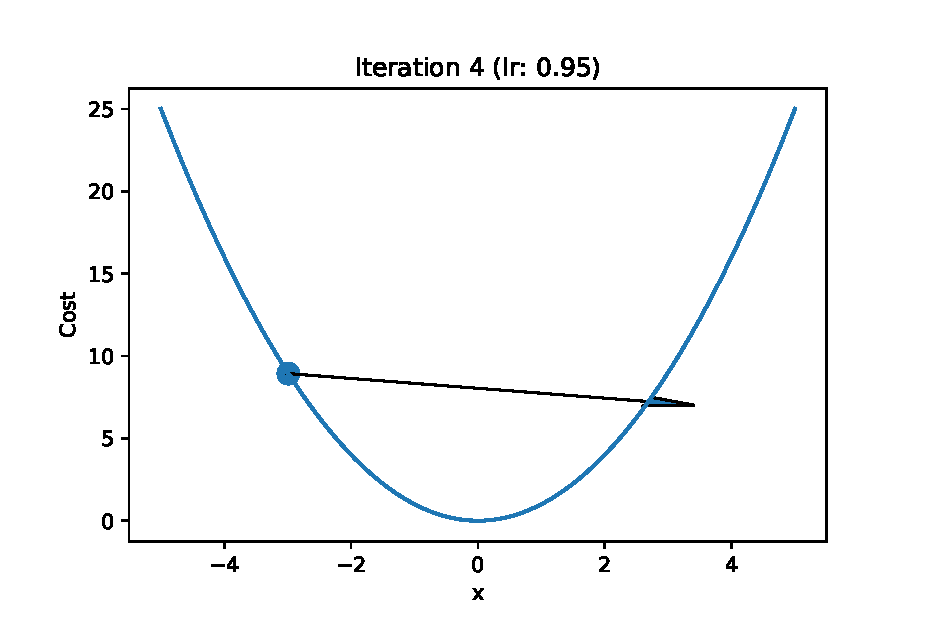
\includegraphics[totalheight=6cm]{gradient-descent/overshooting-4.eps}
		\end{center}
	\end{frame}
	
	\begin{frame}{Overshooting}
		\begin{center}
			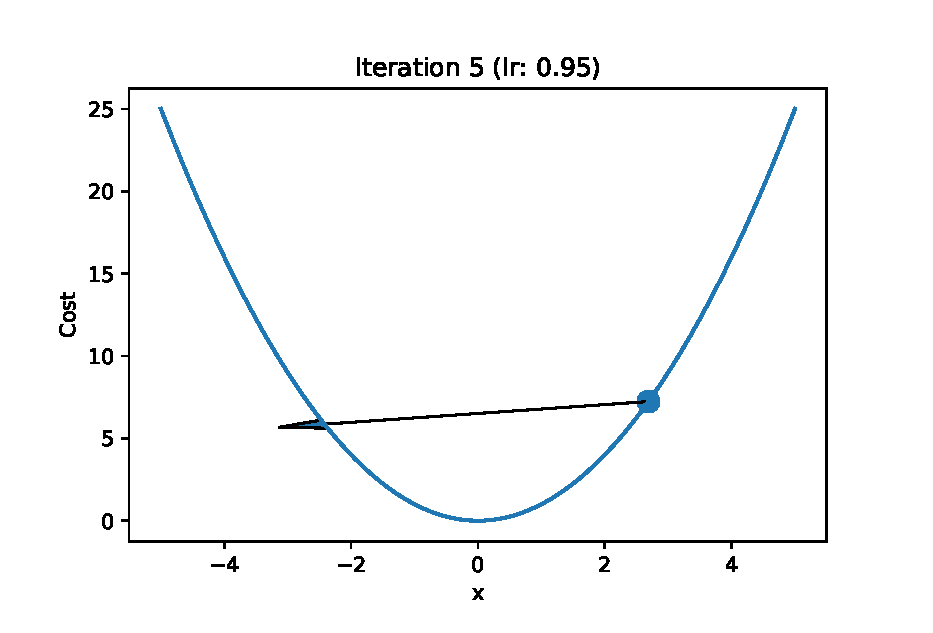
\includegraphics[totalheight=6cm]{gradient-descent/overshooting-5.eps}
		\end{center}
	\end{frame}
	
	\begin{frame}{Overshooting}
		\begin{center}
			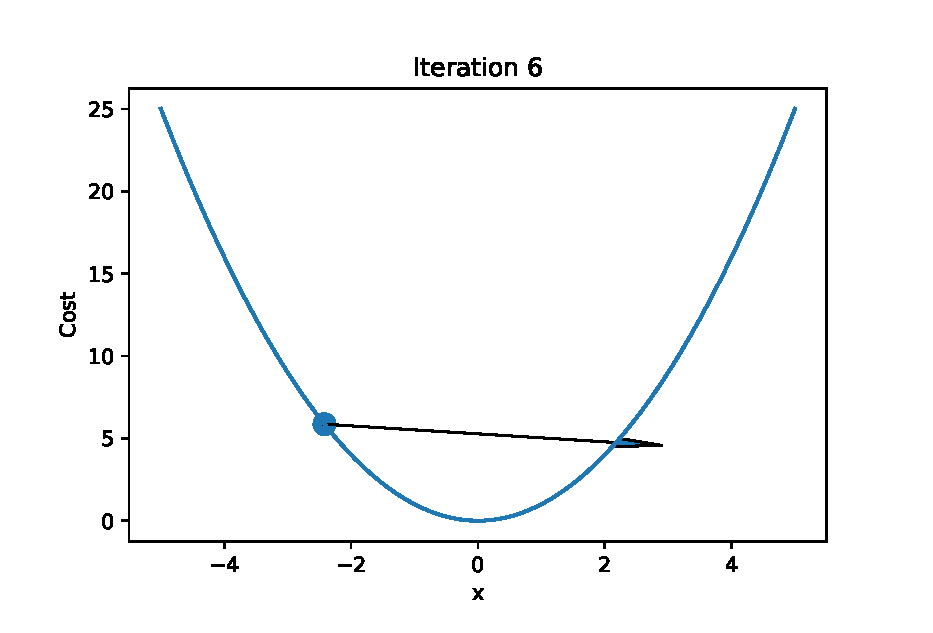
\includegraphics[totalheight=6cm]{gradient-descent/overshooting-6.eps}
		\end{center}
	\end{frame}
	
	\begin{frame}{Overshooting}
		\begin{center}
			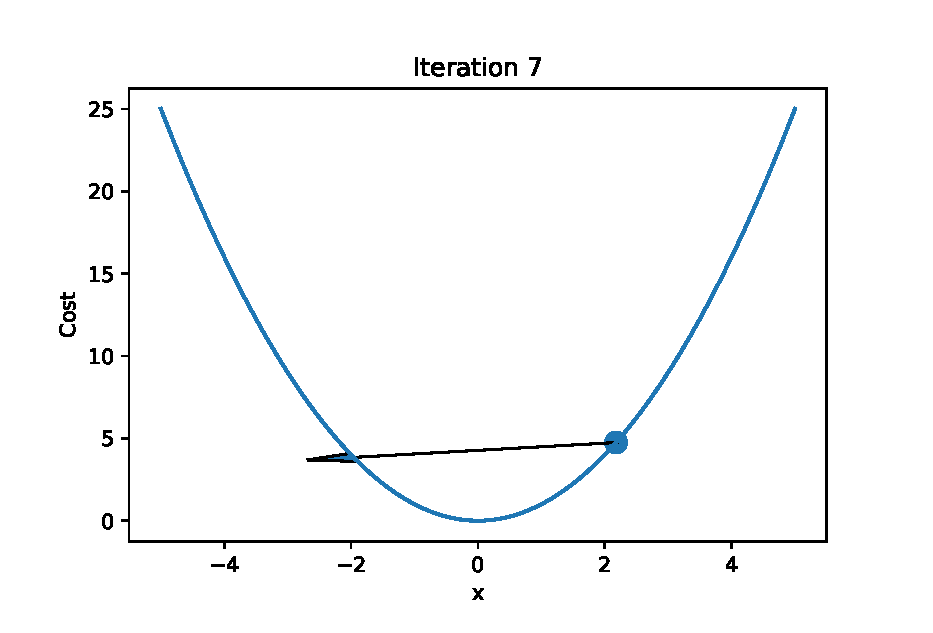
\includegraphics[totalheight=6cm]{gradient-descent/overshooting-7.eps}
		\end{center}
	\end{frame}
	
	\begin{frame}{Overshooting}
		\begin{center}
			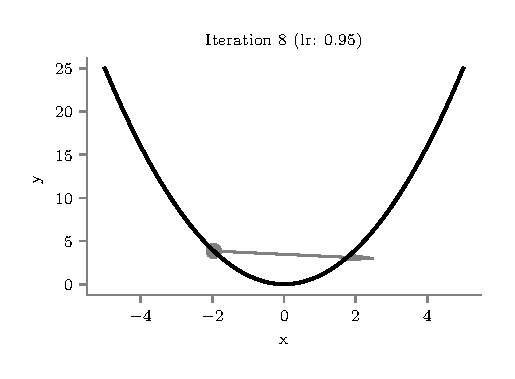
\includegraphics[totalheight=6cm]{gradient-descent/overshooting-8.eps}
		\end{center}
	\end{frame}
	
	\begin{frame}{Overshooting}
		\begin{center}
			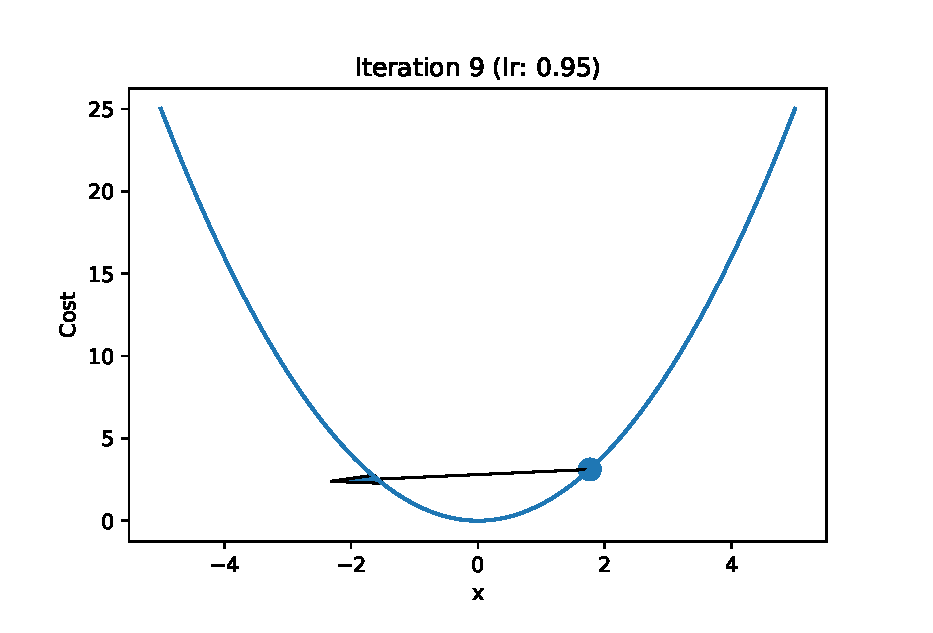
\includegraphics[totalheight=6cm]{gradient-descent/overshooting-9.eps}
		\end{center}
	\end{frame}
	
	\begin{frame}{Overshooting}
		\begin{center}
			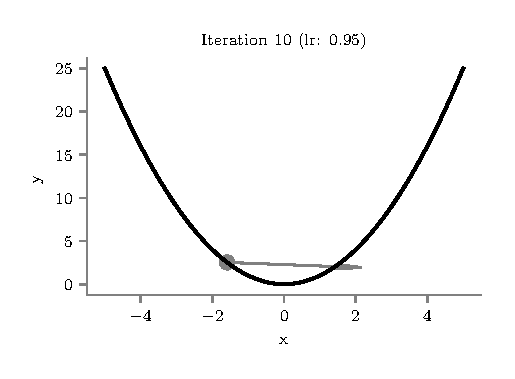
\includegraphics[totalheight=6cm]{gradient-descent/overshooting-10.eps}
		\end{center}
	\end{frame}
	
	\begin{frame}{What if $\alpha$ is very small?}
		Then the rate of convergence is small. It takes more time for a model to reach the minimum cost!
	\end{frame}
	
	\begin{frame}{Slow Convergence}
		\begin{center}
			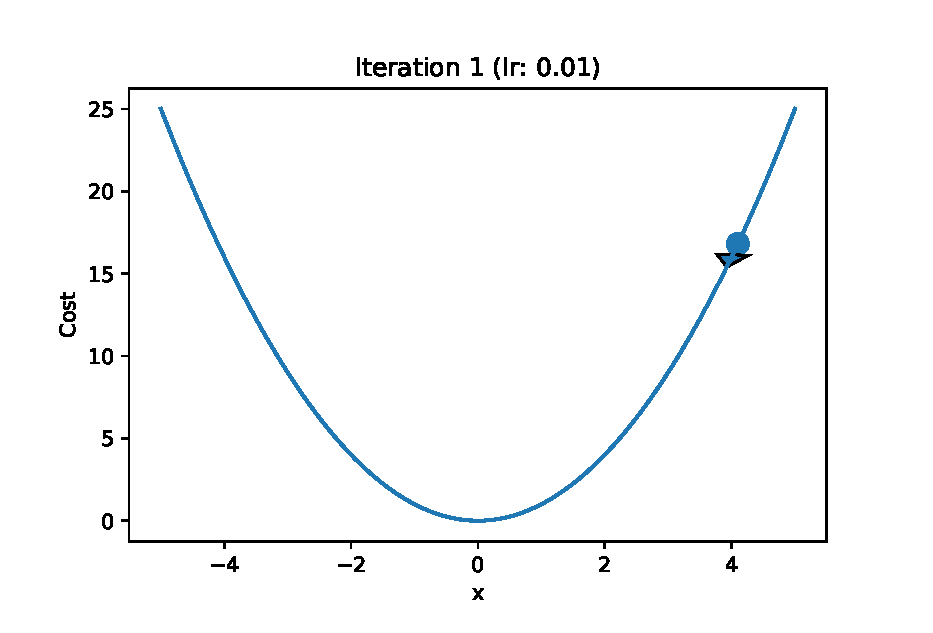
\includegraphics[totalheight=6cm]{gradient-descent/undershooting-1.eps}
		\end{center}
	\end{frame}
	
	\begin{frame}{Slow Convergence}
		\begin{center}
			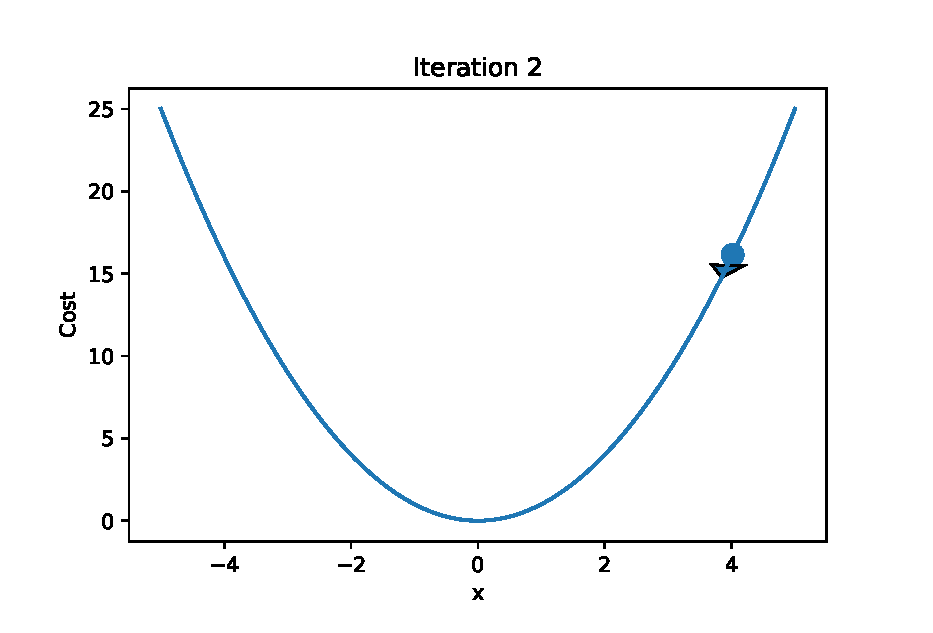
\includegraphics[totalheight=6cm]{gradient-descent/undershooting-2.eps}
		\end{center}
	\end{frame}
	
	\begin{frame}{Slow Convergence}
		\begin{center}
			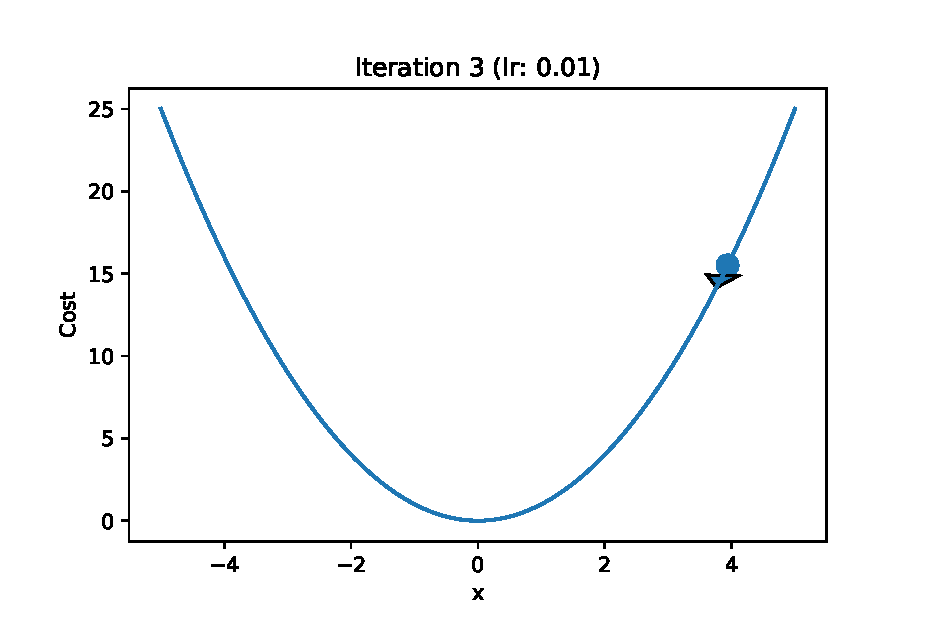
\includegraphics[totalheight=6cm]{gradient-descent/undershooting-3.eps}
		\end{center}
	\end{frame}
	
	\begin{frame}{Slow Convergence}
		\begin{center}
			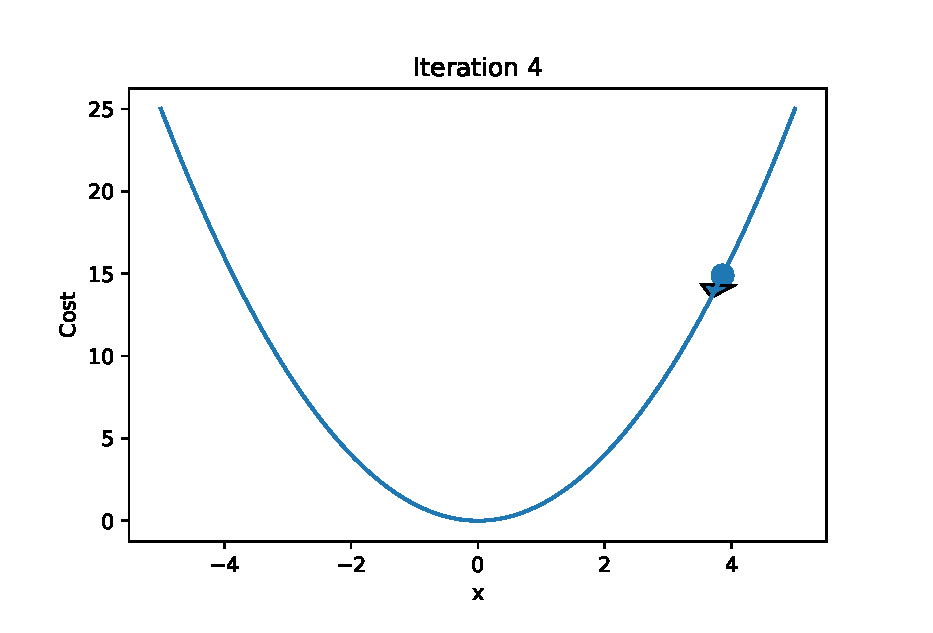
\includegraphics[totalheight=6cm]{gradient-descent/undershooting-4.eps}
		\end{center}
	\end{frame}
	
	\begin{frame}{Slow Convergence}
		\begin{center}
			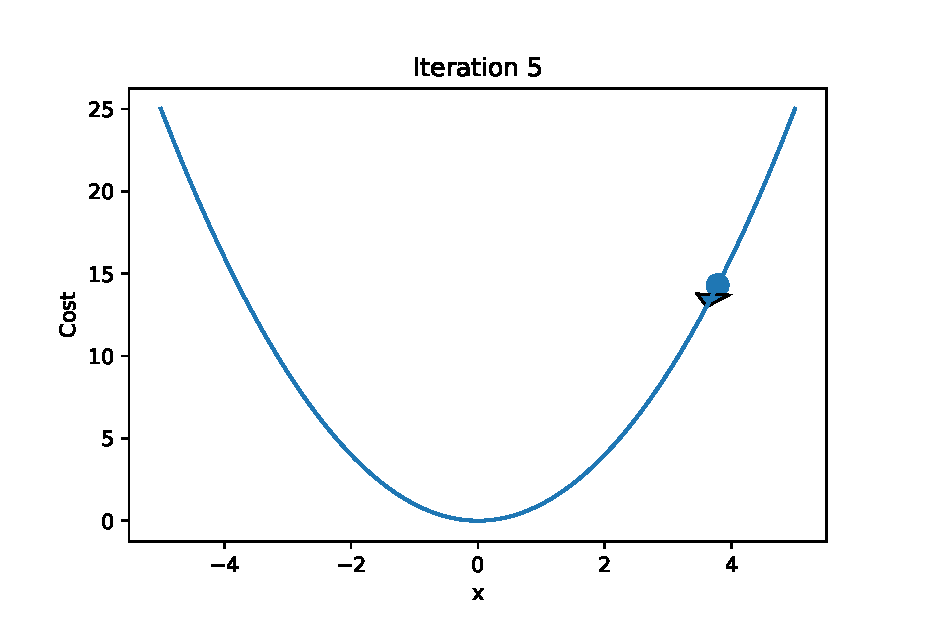
\includegraphics[totalheight=6cm]{gradient-descent/undershooting-5.eps}
		\end{center}
	\end{frame}
	
	\begin{frame}{Slow Convergence}
		\begin{center}
			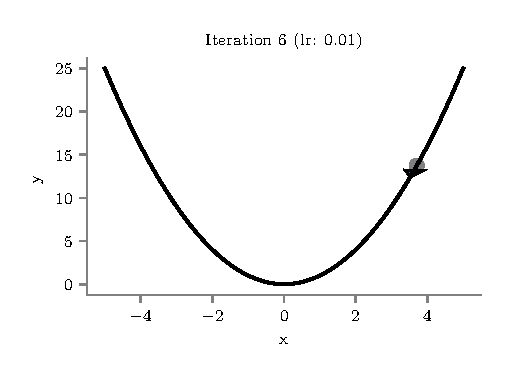
\includegraphics[totalheight=6cm]{gradient-descent/undershooting-6.eps}
		\end{center}
	\end{frame}
	
	\begin{frame}{Slow Convergence}
		\begin{center}
			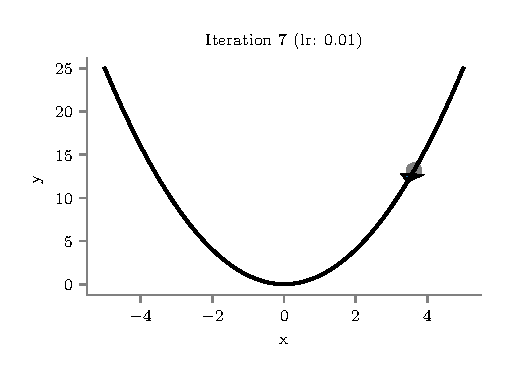
\includegraphics[totalheight=6cm]{gradient-descent/undershooting-7.eps}
		\end{center}
	\end{frame}
	
	\begin{frame}{Slow Convergence}
		\begin{center}
			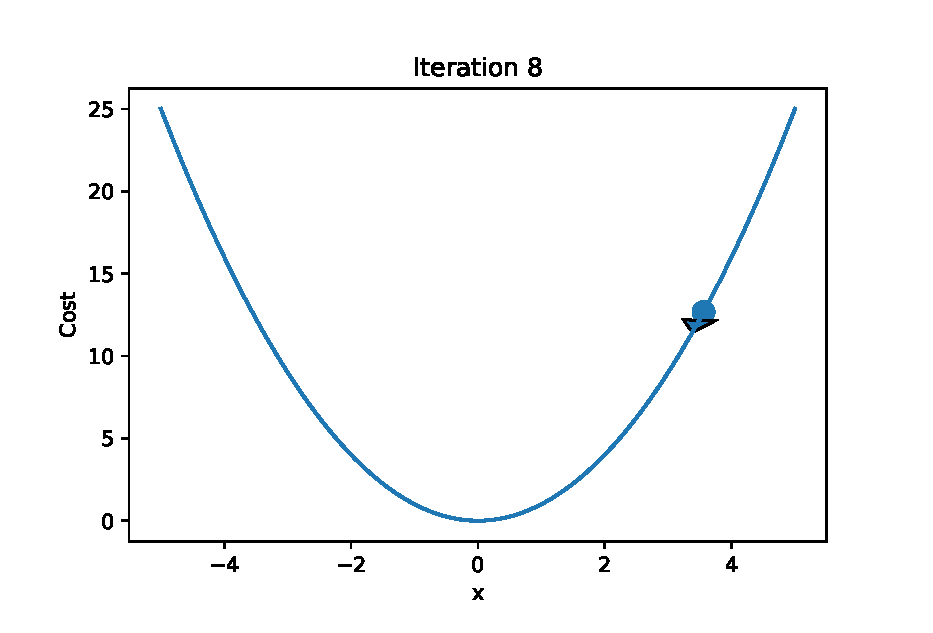
\includegraphics[totalheight=6cm]{gradient-descent/undershooting-8.eps}
		\end{center}
	\end{frame}
	
	\begin{frame}{Slow Convergence}
		\begin{center}
			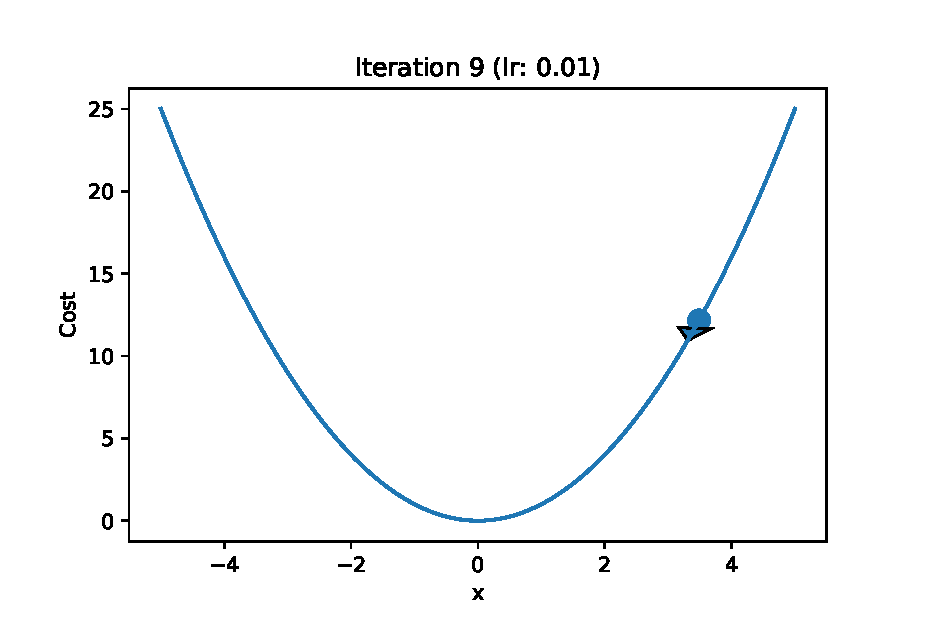
\includegraphics[totalheight=6cm]{gradient-descent/undershooting-9.eps}
		\end{center}
	\end{frame}
	
	\begin{frame}{Slow Convergence}
		\begin{center}
			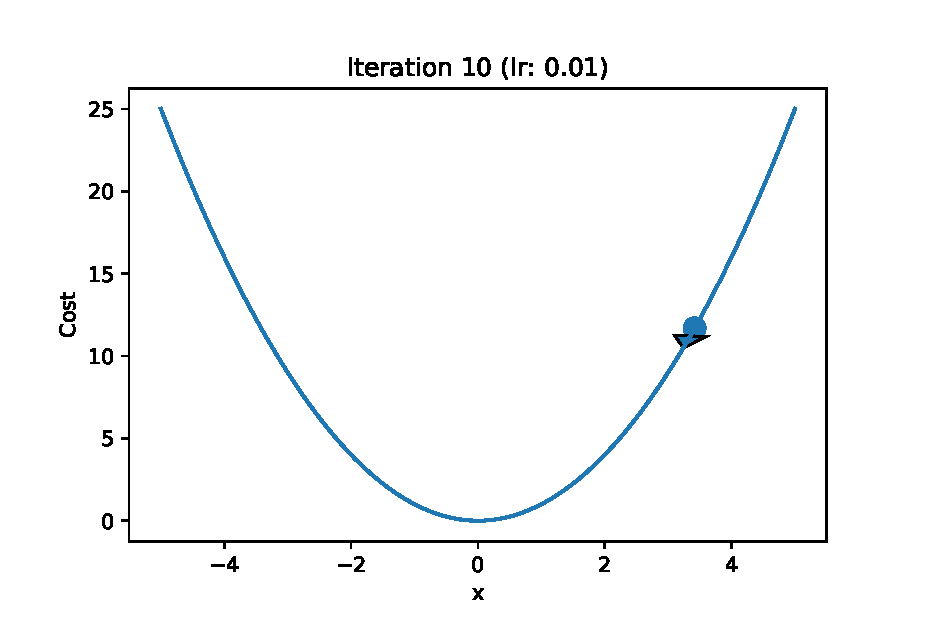
\includegraphics[totalheight=6cm]{gradient-descent/undershooting-10.eps}
		\end{center}
	\end{frame}
	
	
	
	
	\begin{frame}{Gradient Descent for Linear Regression}
		
		\begin{equation*}
		\sum \epsilon_{i}^{2} = \sum (y_{i} - (\theta_{0} + \theta_{1}x_{i}))^{2}
		\end{equation*}
		
	\end{frame}
	
	\begin{frame}{Gradient Descent Algorithm}
		
		Start with random values of $\theta_{0}$ and $\theta_{1}$\\
		Till convergence
		\begin{itemize}
			\item $\theta_{0} = \theta_{0} - \cfrac{\partial}{\partial \theta_{0}} (\sum \epsilon_{i}^{2}) $
			\item $\theta_{1} = \theta_{1} - \cfrac{\partial}{\partial \theta_{1}} (\sum \epsilon_{i}^{2}) $
		\end{itemize}
		
		\textbf{The updates have to be done simultaneously!}
	\end{frame}
	
	\begin{frame}{Gradient Descent Algorithm}
		
		\begin{itemize}
			\item $\cfrac{\partial}{\partial \theta_{0}} (\sum \epsilon_{i}^{2}) = 2\sum (y_{i} - (\theta_{0} + \theta_{1}x{i}))(-1)$
			$\cfrac{\partial}{\partial \theta_{1}} (\sum \epsilon_{i}^{2}) = 2\sum (y_{i} - (\theta_{0} + \theta_{1}x{i}))(-x_{i})$
		\end{itemize}
	\end{frame}
	
	\begin{frame}{Gradient Descent vs SGD}
		\begin{center}
			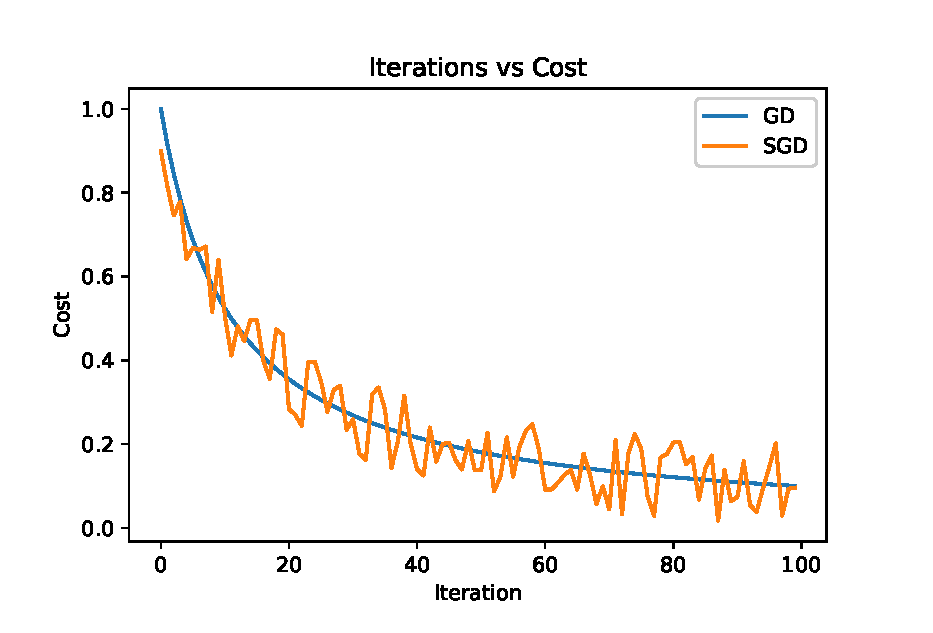
\includegraphics[totalheight=6cm]{gradient-descent/gd-sgd.eps}
		\end{center}
	\end{frame}
	
	
	
	
	\begin{frame}{Gradient Descent vs SGD}
		
		
		
		Vanilla Gradient Descent
		\begin{itemize}
			\item 
			in Vanilla(Batch) gradient descent: We update params after going through all the data 
			\item Smooth curve for Iteration vs Cost
			\item For a single update, it needs to compute the gradient over all the samples, hence takes more time
			
		\end{itemize}
		
		Stochastic Gradient Descent
		\begin{itemize}
			\item In SGD, we update parameters after seeing each each point
			\item Noisier curve for iteration vs cost is much smoother
			\item  For a single update, it computes the gradient over one example. hence lesser time
		\end{itemize}
		
		
	\end{frame}
	
	\begin{frame}{Mini-Batch Gradient Descent}
		
		In mini-batch gradient descent, we compute the gradient over a mini-batch of samples, thereby getting the best of both worlds.
		
	\end{frame}
	
	\begin{frame}{When to use Gradient Descent}
		
		
		Gradient Descent
		\begin{itemize}
			\item Good for online setting(more data)
			\item Good for large data
		\end{itemize}
		
		
		Normal systems
		\begin{itemize}
			\item Good for simple data
			\item No need to worry about learning rates, etc
			\item Non trivial to solve
		\end{itemize}
	\end{frame}
	
	
	
	\begin{frame}{Projected Gradient Descent}
		For the $\theta_{i}$
		
		\begin{equation*}
		\theta_{i} = max(\theta_{i} - \alpha \cfrac{\partial \epsilon (\theta_{0},\theta_{1},...)}{ \nabla  \theta_{i}},0)
		\end{equation*}
	\end{frame}
	
	\begin{frame}{Difference between SSE and MSE}
		
		
		
		\begin{equation*}
		\sum \epsilon_{i}^{2} \textit{ increases as the number of examples increase}
		\end{equation*}
		
		So, we use MSE
		
		\begin{equation*}
		\textit{MSE} = \frac{1}{n} \sum \epsilon_{i}^{2}
		\end{equation*}
		
		Here $n$ denotes the number of samples
		
		
		
	\end{frame}
	
	\begin{frame}{When to Stop iterating?}
		We stop iterating when the MSE at epoch $i$ is close to the loss at MSE at epoch $i+1$.
	\end{frame}
	
\end{document}